\documentclass[main.tex]{subfiles}
\newgeometry{left=25mm, right=25mm, top=20mm, bottom=20mm}
\setcounter{page}{27}


\begin{document}{
    \begin{multicols}{2}
    
    \noindent ника $\tilde a  \tilde a^2_. (\tilde b  \tilde b^2_.)$ равна модулю разности вторых косоугольных координат вершин $\tilde a^1$ и $\tilde a^2$ (соответственно вершин $\tilde b^1$, $\tilde b^2$) и равна единице; действительно:

    \[\left|\sum_{j=1}^{n}a_{j}^{1} - \sum_{j=1}^{n}a_{j}^{2}\right| = \left|\sum_{j=1}^{n}(a_{j}^{1} - a_{j}^{2})\right|=\]
    \[=a_{j}^{2} - a_{j}^{1} = 1 - 0 = 1\]
    
    Итак, треугольники $\tilde a^1_. \tilde a \tilde a^2_.$ и $\tilde b^1_. \tilde b \tilde b^2_.$ равны по двум сторонам и углу между ними. Значит, стороны $\tilde a^1_.\tilde a^2_.$ и $\tilde b^1_.\tilde b^2_.$, являющиеся изображениями ребер куба одного направления, также равны и параллельны - что и требовалось доказать.
    
    Для доказательства \so{свойства} 2) -- непараллельности изображений перпендикулярных ребер куба - достаточно убедиться в непараллельности изображений \textit{базисных} ребер. А последнее очевидно, так как изображения базисных ребер -- это отрезки, соединяющие узел (0, 0) с изображением п вершин \texttt{в е с а} 1 (их номера равны 1, 2, 4, 8,…, $2^n - 1$).
    
   \vspace{4mm}
   
   \noindent\textbf{Заключение}

   \noindentМы доказали возможность косого параллельного проектирования n-мерного куба на плоскость. Заметим, что чертежи кубов, изображенные на рисунках 4, a, б, обладают еще одним свойством: вершины \textit{одинакового веса} лежат на одной прямой, параллельной первому координатному направлению. Это свойство чертежа не является необходимым для параллельного проектирования -оно, например, не имеет места на рисунке 1. Но часто именно это свойство способствует лучшему пониманию внутренней структуры такого чисто алгебраического объекта, каким является n-мерный куб.

    \end{multicols}
}

\vspace{1cm}

\hrule

\vspace{1cm}

\begin{multicols}{2}

    \section*{Встреча \\ с нашими \\ читателями}

    Редакция журнала побывала в гостях у школьников подмосковного города Загорска, в библиотеке профкома Загорского оптико-механического завода. Эта библиотека одна -- из крупнейших в городе, среди ее читателей много школьников, выписывающих наш журнал.

    Встречу вел заместитель главного редактора журнала B. А. Лешковцев. Он рассказал о задачах, которые ставит перед собой «Квант», статьях, которые появятся в журнале в ближайшее время. Школьники в свою очередь высхазали ряд пожеланий редакции, указали разделы математики и физики кото-


    \columnbreak  
    
    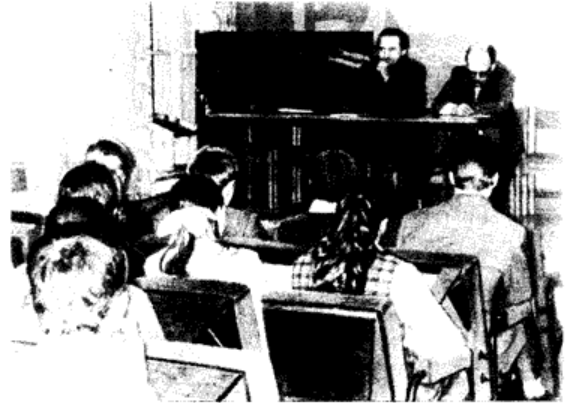
\includegraphics[height=\textheight, width=\linewidth, keepaspectratio]{images/photo.png}

        \begin{multicols}{2}

        \noindent рые их особенно интересуют, подсказали ряд тем для статей. Затем сотрудники редакции ответили на вопросы читателей.
        \columnbreak

        В заключение был проведен небольшой конкурс п по решению задач, победители которогоб были награждены памятными книгами.

        \raggedleft{B. Н. Березин}
        \end{multicols}

\end{multicols}

\hrule

\end{document}